\chapter{Fundamentação Teórica}
Este capítulo apresenta conceitos utilizados no desenvolvimento do trabalho, e portanto necessários para o correto entendimento do mesmo. Os tópicos aqui abordados são, quando necessários, direcionados ao objetivo final do trabalho e por isso podem não representar o universo do conhecimento sobre seu respectivo assunto.

\section{Redes de Computadores}
\label{redes-de-computadores}
A história dos computadores de grande escala começa em fevereiro de 1946 através da invenção do primeiro ``computador integrador numérico eletrônico'' \sigla{ENIAC}{\emph{Electronic Numerical Integrator and Computer}} \cite{Book-Jean2013}. Ele começou a ser desenvolvido anos antes, durante a Segunda Guerra Mundial, com a principal tarefa de auxiliar nos cálculos necessários para o fronte de batalha.

Em meados dos anos 50, com a popularização dos transistores, foi possível realizar uma imensa miniaturização dos circuitos eletrônicos possibilitando a criação de máquinas com altíssimo poder de processamento em um tamanho extremamente reduzido. Além disso, essas máquinas tornaram-se cada vez mais robustas e baratas, fazendo com que a posse e utilização de computadores pudesse ser disseminada, alcançando os patamares atuais.

Neste sentido foi natural a necessidade da troca de informações/dados entre os diversos computadores existentes, o que claramente não representa maiores problemas caso os equipamentos em questão estejam fisicamente perto uns dos outros. Em contrapartida, é fácil imaginar a dificuldade de realização desta tarefa no caso em que estes equipamentos estejam fisicamente distantes. Este é o cerne do problema que motivou a criação das redes de computadores.

Segundo \cite{Book-Kurose2013} uma rede de computadores nada mais é do que uma infraestrutura de comunicação que fornece serviços à aplicações distribuídas através de \emph{links} de comunicação contendo ``chaveadores de pacotes''. Além disso uma rede pode ser essencialmente definida por seu tamanho, topologia e tecnologia de transmissão utilizada \cite{Book-Tanenbaum2003}. A Figura \ref{fig_rede_comunicacao} mostra uma simplificação de uma rede de comunicação onde estas características podem ser encontradas.

\begin{figure}[!htb]
	\centering
	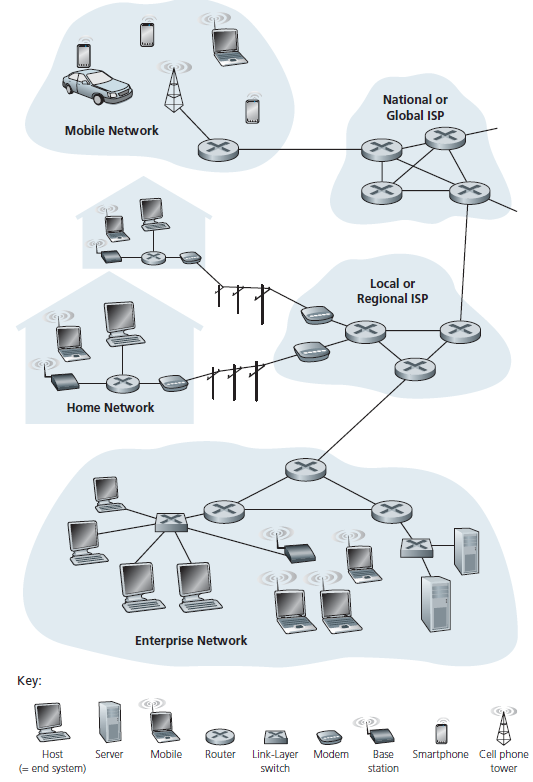
\includegraphics[width=0.6\textwidth]{./figuras/Rede_computadores.png} % <- formatos PNG, JPG e PDF
	\caption[Exemplo de rede de comunicação]{Exemplo de rede de comunicação. Pode-se notar a presença de redes de diferentes tamanhos, topologias e tecnologias de transmissão.}
	\fonte{\cite{Book-Kurose2013}}
	\label{fig_rede_comunicacao}
\end{figure} 

\subsection{Tamanho}
Segundo \cite{Book-Tanenbaum2003} uma \sigla{LAN}{\emph{Local Area Network}} ou Rede Local possui tamanho restrito, e por isso seu desempenho é previsível. Ou seja, os piores tempos de transmissão de pacotes são conhecidos. 

Este tipo de rede pode possuir diversas topologias diferentes e pode ser encontrada nas mais diversas aplicações, desde residenciais, até industriais ou de automação. Uma das suas principais vantagens é a previsibilidade em termos de latência, visto que além de limitada e completamente conhecida ela normalmente não sofre alterações frequentes.

Uma Rede Metropolitana ou \sigla{MAN}{Metropolitan Area Network}, por sua vez, abrange uma cidade. Redes como esta foram inicialmente instaladas para sinais de TV a cabo. Atualmente, esta abordagem é também utilizada por provedores de internet \cite{Book-Tanenbaum2003}.

Uma Rede Geograficamente Distribuída ou \sigla{WAN}{Wide Area Network} abrange uma grande região como um país ou um continente e é responsável pelo roteamento dos pacotes entre as redes origem e destino. A forma e caminho utilizados para enviar as informações neste processo depende do algoritmo de roteamento utilizado. \cite{Book-Tanenbaum2003}

\subsection{Topologia}
Existem diversas formas de realizar a interconexão entre \emph{hosts} (dispositivos finais ou \emph{endpoints}). A topologia da rede depende de como esta interconexão é realizada. De maneira geral, podem-se destacar como mais comuns as topologias em barramento, anel, estrela, árvore e \emph{mesh}.

Uma topologia em barramento compartilha um mesmo meio para diversos \emph{hosts}. Todas as vezes que um deles deseja enviar alguma informação todos os equipamentos a recebem mas apenas o destinatário final a utiliza. Visto que o meio de comunicação é compartilhado, faz-se necessário existir alguma política de controle de acesso ao meio, prevenindo que mais de um \emph{endpoint} envie dados ao mesmo tempo, o que poderia gerar uma ``colisão'' embaralhando os dados de ambas as fontes. Este controle fica sob responsabilidade do protocolo de comunicação utilizado. A Figura \ref{fig_topologia_multiplo_barramento} representa uma rede conectada em barramento, percebe-se que o barramento central é compartilhado entre os diversos dispositivos conectados.

%\begin{figure}[!htb]
	%\centering
	%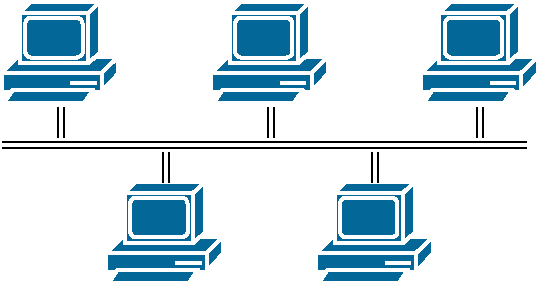
\includegraphics[width=0.2\textwidth]{./figuras/Topologia-Barramento.pdf} % <- formatos PNG, JPG e PDF
	%\caption[Exemplo de topologia em barramento]{Exemplo de topologia conectada em barramento. Percebe-se que o barramento central é compartilhado entre os diversos dispositivos conectados.}
	%\label{fig_topologia_barramento}
%\end{figure}

Na topologia em anel os \emph{hosts} são conectados através de um \emph{link} fechado, criando um anel. Cada estação é responsável por receber os dados em uma porta e encaminhá-los à outra até que este alcance seu destino. Neste tipo de topologia as colisões de dados são menos frequentes, visto que cada enlace do \emph{link} é estabelecido entre apenas dois \emph{hosts}, em contrapartida o protocolo utilizado precisa tratar a dinâmica de recepção e retransmissão de dados entre todos os \emph{links}. Este tipo de rede fornece redundância já que as mensagens trocadas podem ser enviadas por mais de um caminho (sentido horário ou sentido anti-horário). A Figura \ref{fig_topologia_multiplo_barramento_anel} representa uma rede em anel, pode-se perceber que neste caso todos os equipamentos fazem parte da rede e precisam repetir os dados recebidos para os demais.

%\begin{figure}[!htb]
	%\centering
	%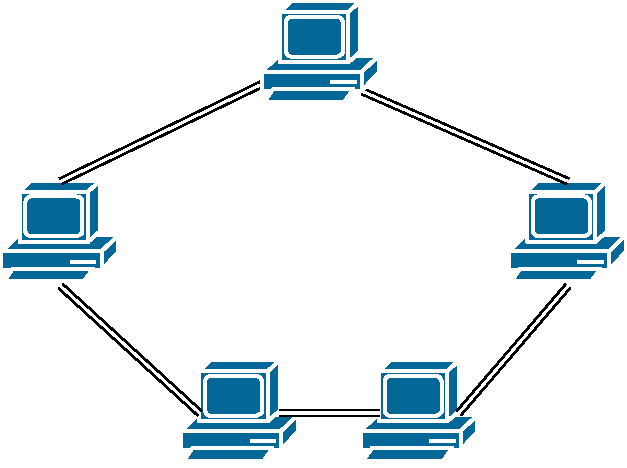
\includegraphics[width=0.2\textwidth]{./figuras/Topologia-Anel.pdf} % <- formatos PNG, JPG e PDF
	%\caption[Exemplo de topologia em anel]{Exemplo de topologia conectada em anel. Percebe-se que todos os equipamentos fazem parte da rede e precisam repetir os dados recebidos para os demais.}
	%\label{fig_topologia_anel}
%\end{figure}

A topologia estrela é muito utilizada em redes sem fio, visto que de maneira geral, todos os \emph{hosts} estão conectados a um ponto de acesso ou \sigla{AP}{Access Point}. Esse tipo de rede também pode ser facilmente encontrada em um meio cabeado, como no caso da utilização dos roteadores/switches residenciais, onde todos os \emph{hosts} são conectados a um mesmo equipamento responsável pela criação de uma LAN e interconexão com uma WAN. A Figura \ref{fig_topologia_multiplo_estrela} representa uma rede de topologia estrela, neste tipo de topologia todos os equipamentos estão ligados a um nó central, neste caso um \emph{switch}.

%\begin{figure}[!htb]
	%\centering
	%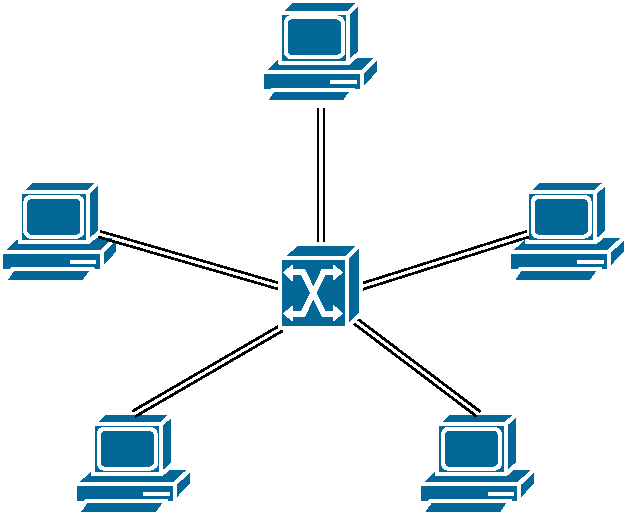
\includegraphics[width=0.2\textwidth]{./figuras/Topologia-Estrela.pdf} % <- formatos PNG, JPG e PDF
	%\caption[Exemplo de topologia em estrela]{Exemplo de topologia conectada em estrela. Percebe-se que todos os equipamentos estão ligados a um nó central, neste caso um \emph{switch}.}
	%\label{fig_topologia_estrela}
%\end{figure}

A topologia em árvore, talvez a mais recorrente em redes de computadores, é assim chamada pois pode ser reconhecida pelo seu aspecto, onde o nó central representa a base da árvore e os diversos \emph{hosts} representam suas folhas (normalmente representada como uma árvore invertida). Basicamente trata-se de uma estrutura hierárquica de conexão entre várias redes e/ou sub-redes. A Figura \ref{fig_topologia_multiplo_arvore} ilustra esse tipo de topologia. Percebe-se que a topologia assemelha-se à interconexão de várias sub-redes através de equipamentos dedicados.

%\begin{figure}[!htb]
	%\centering
	%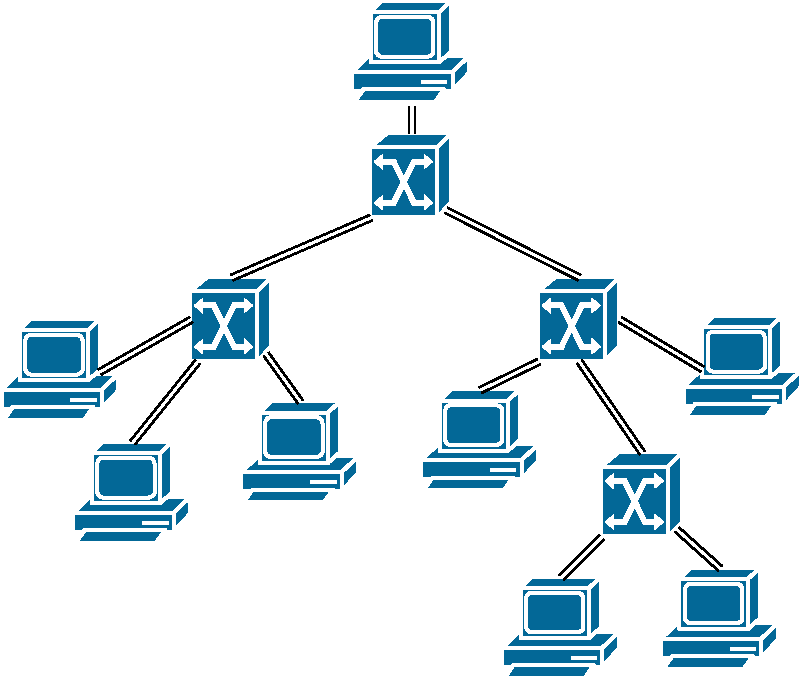
\includegraphics[width=0.2\textwidth]{./figuras/Topologia-Arvore.pdf} % <- formatos PNG, JPG e PDF
	%\caption[Exemplo de topologia em árvore]{Exemplo de topologia conectada em árvore. Percebe-se que a topologia assemelha-se à interconexão de várias sub-redes através de equipamentos dedicados.}
	%\label{fig_topologia_arvore}
%\end{figure}

A topologia em malha ou \emph{mesh} por sua vez, é caracterizada pela criação de uma rede grandemente (podendo chegar a ser plenamente) interconectada, formando diversos caminhos redundantes para a interligação entre a origem e o destino das mensagens. Fato que confere a este tipo de rede um elevado grau de disponibilidade, visto que mesmo em caso de falha de equipamentos ou da infraestrutura a comunicação não é necessariamente comprometida. A Figura \ref{fig_topologia_multiplo_mesh} ilustra uma rede \emph{mesh}. É possível notar que existem diversas rotas redundantes devido aos vários links estabelecidos entre os equipamentos da rede. Da mesma forma, nota-se que neste tipo de topologia de rede existem custos atrelados ao roteamento, encaminhamento e processamento de pacotes já que, excluindo-se a situação em que o ponto origem e o destino da comunicação seja vizinhos (diretamente ligados um ao outro), será invariavelmente necessária a repetição de pacotes por parte de nós intermediários para o estabelecimento da comunicação.

%\begin{figure}[!htb]
	%\centering
	%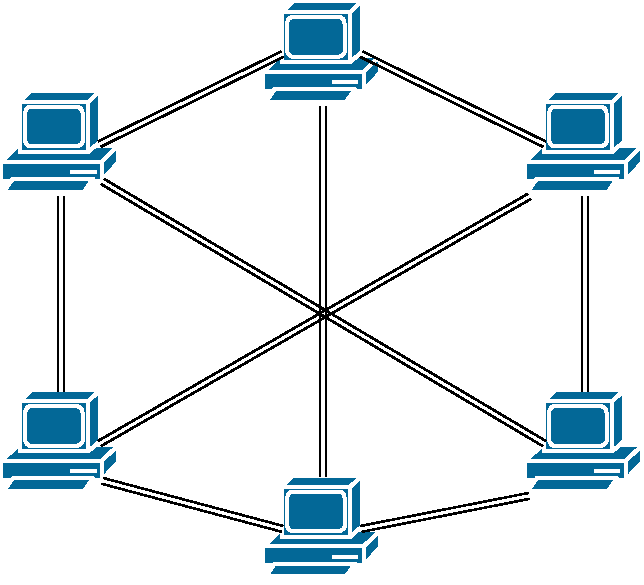
\includegraphics[width=0.2\textwidth]{./figuras/Topologia-Mesh.pdf} % <- formatos PNG, JPG e PDF
	%\caption[Exemplo de topologia em \emph{mesh}]{Exemplo de topologia conectada em \emph{mesh}. Percebe-se existem diversas rotas redundantes devido aos vários links estabelecidos entre os equipamentos da rede.}
	%\label{fig_topologia_mesh}
%\end{figure}

\begin{figure}[t!]
	\centering
	\begin{subfigure}[t]{0.4\textwidth}
		\centering
		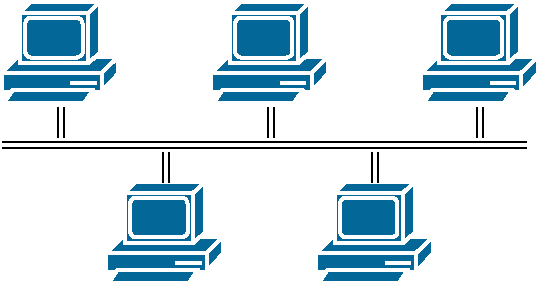
\includegraphics[width=4cm]{./figuras/Topologia-Barramento.pdf} % <- formatos PNG, JPG e PDF
		\caption{Topologia em barramento.}
		\label{fig_topologia_multiplo_barramento}
	\end{subfigure}%
	~
	\begin{subfigure}[t]{0.4\textwidth}
		\centering
		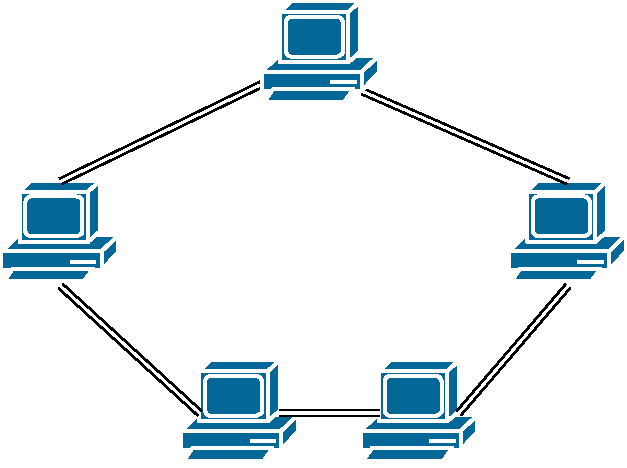
\includegraphics[width=4cm]{./figuras/Topologia-Anel.pdf} % <- formatos PNG, JPG e PDF
	\caption{Topologia em anel.}
	\label{fig_topologia_multiplo_barramento_anel}
	\end{subfigure}
	~
	\begin{subfigure}[t]{0.4\textwidth}
		\centering
		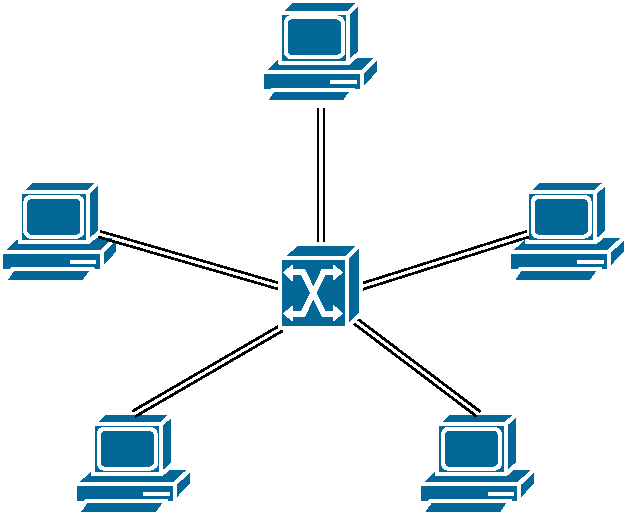
\includegraphics[width=4cm]{./figuras/Topologia-Estrela.pdf} % <- formatos PNG, JPG e PDF
	\caption{Topologia em estrela.}
	\label{fig_topologia_multiplo_estrela}
	\end{subfigure}
	~
	\begin{subfigure}[t]{0.4\textwidth}
		\centering
		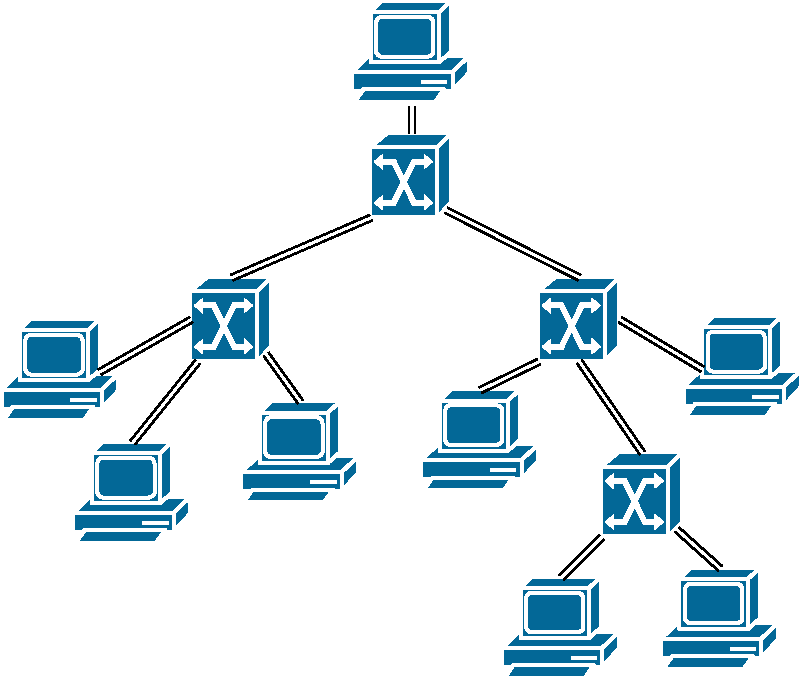
\includegraphics[width=4cm]{./figuras/Topologia-Arvore.pdf} % <- formatos PNG, JPG e PDF
	\caption{Topologia em árvore.}
	\label{fig_topologia_multiplo_arvore}
	\end{subfigure}
	~
	\begin{subfigure}[t]{0.4\textwidth}
		\centering
		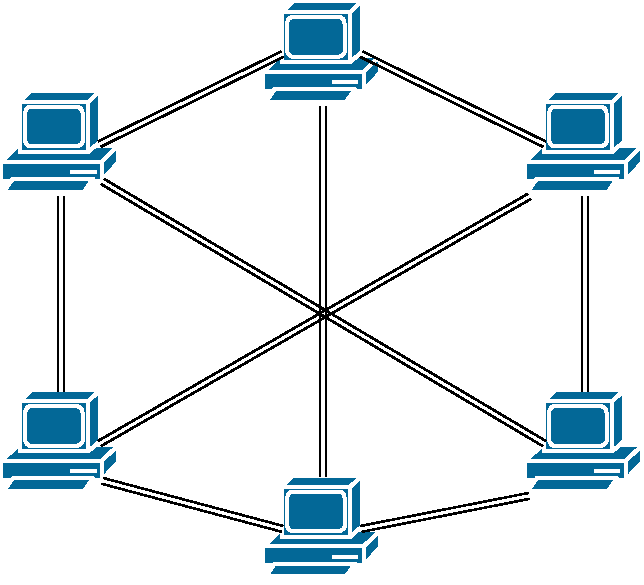
\includegraphics[width=4cm]{./figuras/Topologia-Mesh.pdf} % <- formatos PNG, JPG e PDF
	\caption{Topologia em \emph{mesh}.}
	\label{fig_topologia_multiplo_mesh}
	\end{subfigure}
	\caption{Tipos básicos de topologia}
	\label{fig_topologia_multiplo}
\end{figure}

\subsection{Tecnologia de Transmissão}
A tecnologia de transmissão está diretamente ligada ao meio físico utilizado, que não precisa ser necessariamente construído em cabos metálicos. Podem ser utilizados fibras ópticas, enlaces de micro-ondas, ondas infravermelhas, satélites de comunicação, entre outros \cite{Book-Tanenbaum2003}. 

Além disso, as redes de computadores podem, e comumente são, criadas através da interconexão de redes híbridas, ou seja, diferentes sub-redes criadas com tecnologias de transmissão distintas. Essas redes por sua vez têm diferentes taxas de transmissão e valores típicos de latência e demais parâmetros aos quais todos os pacotes que as atravessarem estarão submetidos \cite{Book-Kurose2013} assim como pode-se verificar no exemplo da Figura \ref{fig_rede_comunicacao}. Logo, quando é necessário realizar uma comunicação entre \emph{hosts} em redes que utilizam tecnologias de transmissão diferentes é necessária a existência de algum tipo de mecanismo para regulação da velocidade de transferência de informação, assim como políticas de garantia de entrega dos dados. Estes mecanismos são algumas das responsabilidades básicas dos protocolos de comunicação como o TCP/IP.

\section{Comutadores Ópticos}
A comunicação em redes ópticas é feita através da modulação de sinais luminosos, cada um desses sinais possui uma frequência diferente (usualmente também chamada de cor do sinal) o que implica em diferentes comprimentos de onda (\simbolo{$\lambda$}{comprimento de onda}). Redes complexas e com grande número de $\lambda$s  como as redes ópticas atuais, possuem em seus nós centrais equipamentos conhecidos como comutadores ópticos, também chamados de \sigla{OXC}{Optical Cross Connect}. 

Os OXCs podem realizar roteamento interno de sinais de maneira puramente óptica, puramente elétrica ou até mesmo híbrida \cite{Book-Ramaswami2010}. Existem basicamente três diferentes classificações de equipamentos OXC, os opacos, os transparentes e os translúcidos.
%Usar Optical Networks pagina 488

OXCs opacos são assim chamados por impedirem a passagem direta da luz, ou seja, o roteamento que esse tipo de equipamento oferece é realizado no domínio elétrico. Para isso todos os sinais que entram no equipamento são convertido em sinais elétricos e enviados a um \emph{switch} ou processador eletrônico que fará o devido roteamento, para que então esses sinais sejam novamente convertidos em sinais ópticos através da utilização de \emph{transceivers} e lasers. Este tipo de equipamento é amplamente empregado nas redes ópticas atuais e são muitas vezes conhecidos como \sigla{OEO}{Optical-Electrical-Optical} ou Óptico-Elétrico-Óptico em tradução livre.

Equipamentos OXC opacos possuem o inconveniente de que a circuitaria eletrônica utilizada para o processamento dos dados acaba por limitar a banda do sinal, ou seja, seu \emph{throughput}. Existem diversas razões para esta limitação sendo as principais delas as conversões de meio necessárias e o poder de processamento do próprio equipamento. Apesar disso, a grande vantagem deste tipo de equipamento reside no custo benefício, já que ele possibilita a regeneração do sinal óptico a cada nó da rede, visto que o sinal precisa ser recriado, e o controle e obtenção de métricas relativas à comunicação transportada por ele, o que tem grande valor para a gerência da rede, além de normalmente ter um custo atrativo quando comparado aos outros modelos.  

OXCs transparentes por sua vez, são assim chamados por não interromperem o sinal de luz que os transpassa. Esse tipo de equipamento tem a capacidade de realizar a separação dos comprimentos de onda de luz e seu devido encaminhamento ou roteamento para a interface desejada. 

Em linhas gerais, a luz que chega ao equipamento (composta por diferentes $\lambda$s) é demultiplexada de acordo com a sua cor ou $\lambda$, direcionada para a saída desejada e unida aos demais sinais luminosos da respectiva saída através de um multiplexador, para então serem enviados através de uma fibra óptica. 

Percebe-se que este tipo de equipamento faz a divisão e roteamento de luz em grande parte de maneira passiva, alterando o menos possível os sinais que por ele transitam (normalmente o efeito mais significativo sobre o sinal está relacionado à potência e separação de $\lambda$s do mesmo). Isto implica basicamente em dois fatores, por um lado a não limitação de banda do sinal garante altíssima performance, por outro a não demodulação/interpretação do sinal impede a obtenção de métricas de qualidade ou controle sobre a comunicação. Além disso, estes equipamentos costumam ter sua performance grandemente atrelada a dispositivos sensíveis, como filtros internos, o que acarreta em um custo final elevado. Razões estas que impedem sua ampla utilização em redes ópticas de grande porte. Normalmente esse tipo de tecnologia pode ser facilmente encontrada em alguns filtros e \emph{splitters} especiais. A Figura \ref{fig_oxc_optico} contém o diagrama básico de um OXC transparente. 

\begin{figure}[!htb]
	\centering
	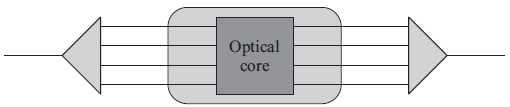
\includegraphics[width=0.5\textwidth]{./figuras/OXC-Optico.png} % <- formatos PNG, JPG e PDF
	\caption[Exemplo básico de OXC óptico]{Exemplo básico de um equipamento OXC transparente. Percebe-se que o sinal de entrada é apenas repassado à respectiva saída sem nenhuma outra intervenção.}
	\fonte{\cite{Book-Ramaswami2010}}
	\label{fig_oxc_optico}
\end{figure}

Por fim, um OXC translúcido traduz-se em um equipamento que representa um compromisso entre os dois tipos anteriores. Ou seja, um equipamento de roteamento em redes ópticas que tem a capacidade de processamento de pacotes e de chaveamento de luz. Este tipo de equipamento, apesar de não ser comumente encontrado, é o foco do presente trabalho.

A proposta que será detalhadamente descrita no Capítulo \ref{capitulo_proposta} aborda a utilização de equipamento óptico similar a um OXC translúcido através da utilização de chaveadores ópticos ou \emph{switches} ópticos.

Chaveadores ópticos são componentes capazes de desviar um feixe luminoso através da utilização de um prisma refletor. A Figura \ref{fig_chaveador_optico} mostra o diagrama interno simplificado de um chaveador óptico, percebe-se que seu funcionamento é análogo ao de um relé elétrico.

\begin{figure}[!htb]
	\centering
	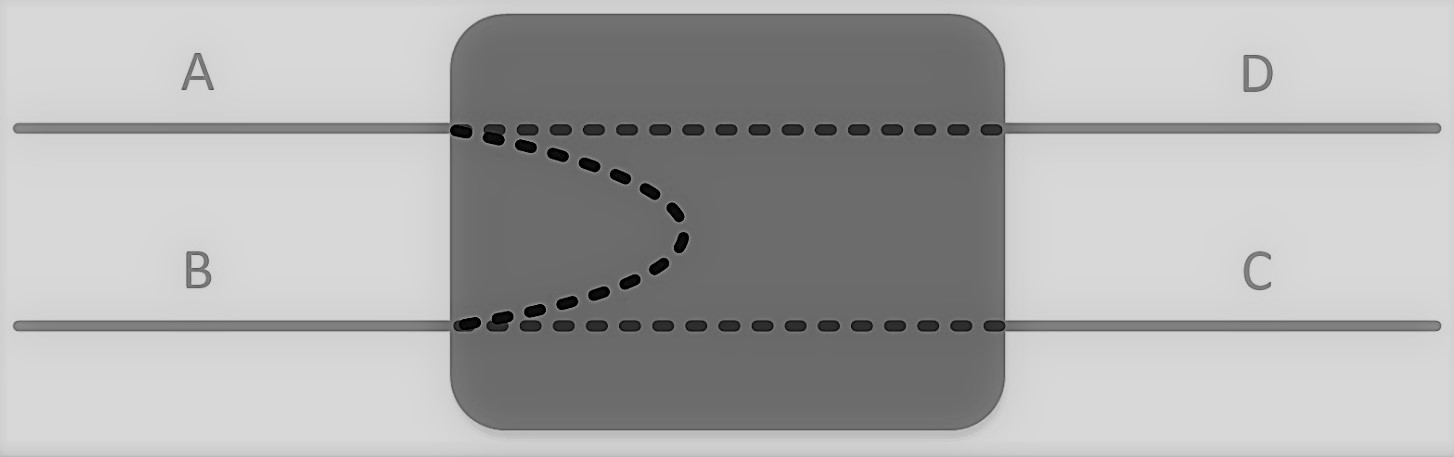
\includegraphics[width=0.5\textwidth]{./figuras/Switch_optico.jpg} % <- formatos PNG, JPG e PDF
	\caption[Exemplo básico chaveador óptico]{Diagrama interno simplificado de um chaveador óptico. Em um estado este componente transmite bidirecionalmente a luz da interface A para D e B para C, quando acionado ele transmite bidirecionalmente a luz da interface A para B.}
	\fonte{Adaptado de \cite{Accelink2014}}
	\label{fig_chaveador_optico}
\end{figure}

É importante ressaltar que um chaveador óptico em si é um componente essencialmente passivo. Quando o prisma refletor interno é acionado a luz passa a ser refletida para a saída sem sofrer outro tipo de influência, ou seja, ela é apenas desviada. Entretanto a utilização de um chaveador óptico em um equipamento OEO pode conferir-lhe a capacidade de desviar sinais ópticos caso necessário, surgindo assim um equipamento de roteamento que pode ser classificado como sendo um OXC translúcido. 

\section{Grafos}
\label{chap_grafos}
Grafos são em essência a representação gráfica de interligação entre diferentes pontos, na matemática a teoria dos grafos é a ciência que estuda as relações entre um conjunto de objetos.

Os grafos são representados por vértices conectados através de arestas (que representam a relação entre os vértices). Caso as arestas sejam orientadas (possuam sentido) o grafo é denominado direcionado, além disso, cada aresta pode conter um peso normalmente indicado no próprio grafo. Os grafos utilizados no presente documento são simples, ou seja, não englobam aqueles que possuem duas arestas diferentes com os mesmo par de pontas (ou seja, não contém arestas paralelas) ou arestas com pontas coincidentes (não contém laços) \cite{Man-Feofiloff2011}. Os tipos de grafos mais comuns são:

\begin{itemize}
	\item Grafo simples: grafo não direcionado, sem arestas paralelas e sem laços;
	\item Grafo direcionado: similar ao grafo simples, porém com arestas direcionadas;
	\item Grafo conexo: um grafo pode ser dito conexo se sempre for possível estabelecer um caminho de qualquer vértice para qualquer outro vértice.
\end{itemize}

A Figura \ref{fig_tipos_grafos} representa os tipos básicos de grafo descritos. Pode-se perceber que o grafo representado na Figura \ref{fig_grafo_simples} possui 5 vértices interligados através de arestas não direcionadas, logo este grafo pode ser classificado com um grafo simples e conexo visto que todos os nós são alcançáveis à partir de qualquer um deles. O grafo da Figura \ref{fig_grafo_direcionado} por sua vez possui arestas direcionadas, podendo ser classificado como um grafo direcionado e conexo. Além disso é possível ver um número em cada uma das arestas representando o peso das mesmas. Por fim, no grafo da Figura \ref{fig_grafo_desconexo} pode-se verificar que nem todos os vértices são alcançáveis à partir de qualquer outro vértice, logo este é um grafo desconexo.

\begin{figure}[t!]
	\centering
	\begin{subfigure}[t]{0.3\textwidth}
		\centering
		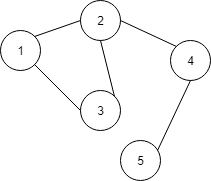
\includegraphics[width=4cm]{./figuras/grafo-simples.png} % <- formatos PNG, JPG e PDF
		\caption{Grafo simples.}
		\label{fig_grafo_simples}
	\end{subfigure}%
	~
	\begin{subfigure}[t]{0.3\textwidth}
		\centering
		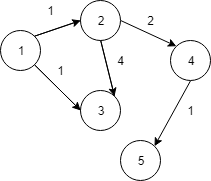
\includegraphics[width=4cm]{./figuras/grafo-direcionado.png} % <- formatos PNG, JPG e PDF
	\caption{Grafo direcionado.}
	\label{fig_grafo_direcionado}
	\end{subfigure}
	~
	\begin{subfigure}[t]{0.3\textwidth}
		\centering
		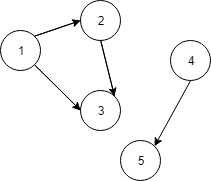
\includegraphics[width=4cm]{./figuras/grafo-desconexo.png} % <- formatos PNG, JPG e PDF
	\caption{Grafo desconexo.}
	\label{fig_grafo_desconexo}
	\end{subfigure}
	\caption{Tipos básicos de grafos}
	\label{fig_tipos_grafos}
\end{figure}

Existem outras convenções para representações de grafos, algumas delas são especialmente úteis para computação, como por exemplo as representações por adjacência visto que, nesta abordagem, a relação entre os vértices pode ser descrita em formato de lista. Dois vértices podem ser considerados adjacentes quando existe uma aresta entre eles. No grafo da Figura \ref{fig_grafo_simples} por exemplo pode-se considerar que os vértices 1 e 2 são adjacentes enquanto os vértices 1 e 5 não são.

Além disso, vale a pena ressaltar o conceito de valência ou grau de um vértice, que nada mais é que o número de arestas incidentes a ele. Utilizando mais uma vez o grafo representado na Figura \ref{fig_grafo_simples} pode-se dizer que os vértices 1, 3 e 4 têm valência 2; o vértice 2 tem valência 3 e o vértice 5 tem valência 1.

Outro conceito importante para o presente trabalho é o de Árvore de extensão ou Árvore de dispersão (\emph{spanning tree} - normalmente o termo em inglês é mais utilizado), que pode ser traduzido como sendo o subconjunto de arestas de um grafo formando uma árvore que contém todos os vértices do grafo inicial. Como desdobramento deste conceito, pode-se facilmente definir a árvore de extensão mínima, árvore de geração mínima ou ainda \emph{minimal spanning tree} como sendo o subconjunto de arestas de menor peso total contendo todos os vértices do grafo inicial (supondo um grafo com arestas contendo pesos) \cite{Eppstein1996}.
%avaliar onde colocar a referencia https://www.ics.uci.edu/~eppstein/pubs/Epp-TR-96-16.pdf
%busca em grafos https://pt.wikipedia.org/wiki/Teoria_dos_grafos

Os grafos, têm diversas aplicações e podem ser usados para representar uma grande variedade de problemas e situações, normalmente eles conseguem modelar de maneira satisfatória alguns dos problemas dos campos da matemática, informática, engenharia, química e outras áreas. De maneira geral, uma das aplicações mais comuns é a utilização de grafos para a descoberta de caminhos entre diferentes pontos, representados como vértices, do grafo em questão. Um caminho em um grafo pode ser definido como uma sequência de vértices de maneira que entre cada um dos vértices listados existe uma aresta para o vértice seguinte, sendo que o custo deste caminho é a soma dos custos das arestas utilizadas.

Existem vários algoritmos de busca em grafos. Considerando-se grafos finitos, sempre é possível percorrer de modo sistemático todos os vértices e arestas existentes. Desta forma é possível também encontrar o menor caminho disponível (menor custo) entre dois vértices. De maneira geral existem dois modos básicos para percorrer um grafo, ``Busca em Largura'' ou \sigla{BFS}{\emph{Breadth-First Search}}; quando durante a procura de um vértice específico os vértices do grafo são visitados respeitando-se os níveis do mesmo;  e ``Busca em profundidade'' ou \sigla{DFS}{\emph{Depth-first search}}; quando durante a procura de um vértice específico todos os nós de um ramo são visitados antes dos vértices do mesmo nível. A Figura \ref{fig-busca-grafo} ilustra a diferença básica entre os dois modos.

\begin{figure}[t!]
	\centering
	\begin{subfigure}[t]{0.4\textwidth}
		\centering
		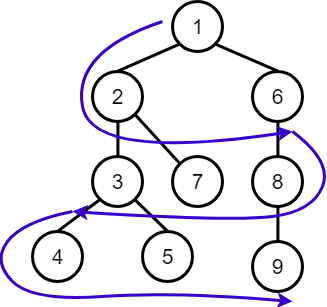
\includegraphics[height=4cm]{./figuras/BFS.png} % <- formatos PNG, JPG e PDF
		\caption{BFS}
		\label{fig_BFS}
	\end{subfigure}%
	~
	\begin{subfigure}[t]{0.4\textwidth}
		\centering
		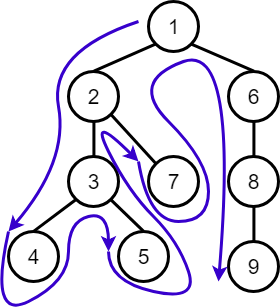
\includegraphics[height=4cm]{./figuras/DFS.png} % <- formatos PNG, JPG e PDF
	\caption{DFS}
	\label{fig_DFS}
	\end{subfigure}
	\caption[Busca em Profundidade vs Largura]{Comparação básica entre busca em profundidade e largura. Em \ref{fig_BFS} pode-se notar que os vértices visitados são prioritariamente do mesmo nível em detrimento aos níveis mais baixos. Em \ref{fig_DFS} pode-se notar que todos os vértices de um ramo são visitados antes que o próximo seja explorado.}
	\label{fig-busca-grafo}
\end{figure}

%https://pt.wikipedia.org/wiki/%C3%81rvore_de_extens%C3%A3o
Dentre os algoritmos mais utilizados para busca em grafos destacam-se, neste documento, dois principais que terão grande aderência ao conteúdo aqui abordado. 

\subsection{Algoritmo de Dijkstra}
%https://pt.wikipedia.org/wiki/Algoritmo_de_Dijkstra
O algoritmo de Dijkstra foi criado por Edsger Dijkstra em 1956. Ele é aplicável a grafos com múltiplos caminhos. À partir da estrutura inicial do grafo e de um vértice raiz, ele é capaz de extrair uma estrutura de árvore com apenas um caminho para cada vértice destino, selecionando para tal, os caminhos menos custosos. Ou seja, com o menor custo até a raiz \cite{Dijkstra1959}.

\subsection{Algoritmo de Prim} 
\label{subsection-algoritmo-prim}
%https://en.wikipedia.org/wiki/Prim%27s_algorithm
O algoritmo de Prim foi desenvolvido por  Vojtech Jarník em 1930 e posteriormente otimizado por Robert C. Prim em 1957 e Edsger Dijkstra em 1959, razão pela qual é também chamado de algoritmo Prim–Dijkstra. Ele é utilizado para encontrar um conjunto de arestas que formam uma árvore contendo todos os vértices de um grafo cujo peso total (soma dos pesos individuais de todas as arestas) é mínimo, formando dessa forma uma árvore geradora mínima \cite{Prim1957}.

\subsection{Algoritmo de Busca de Custo Uniforme}

A Busca de Custo Uniforme é na verdade um algoritmo de busca em grafos que estende o algoritmo de Busca em Largura, representado na Figura \ref{fig_BFS}, de modo a sempre encontrar a solução ótima para qualquer valor de passo (peso) através da expansão do nó com menor custo de caminho \cite{Book-Russell2018}. Em outras palavras o algoritmo de Busca de Custo Uniforme é um tipo de busca em grafos com garantia de otimalidade, visto que é um algoritmo exaustivo. Ou seja, avalia todas as opções até a obtenção do ótimo.

Este algoritmo apresenta um bom custo benefício ao comparar sua complexidade espacial (quantidade de memória utilizada) e temporal (tempo necessário para execução) com a garantia de otimalidade (obtenção do custo ótimo), visto que sua implementação é muito similar ao algoritmo utilizado na BFS.

\section{Protocolos de Roteamento}
\label{cap_protocolos_de_roteamento}
Esta seção destina-se à discussão de alguns dos conceitos de protocolos de roteamento, tendo enfoque no protocolo recorrentemente utilizado no cenário descrito.

\subsection{Protocolos de Roteamento Relacionados}%\subsection{Definição de Protocolo}
Assim como no mecanismo formal de troca de informações entre humanos, um protocolo de comunicação é o que estabelece as regras básicas para troca de dados entre máquinas. Segundo \cite{Book-Kurose2013} um procolo de comunicação define o formato e a ordem das mensagens trocadas entre duas ou mais entidades, assim como as ações necessárias para que esses dados sejam corretamente recebidos/enviados. A Figura \ref{fig_explicacao_protocolo} exemplifica este paralelo.

\begin{figure}[!htb]
	\centering
	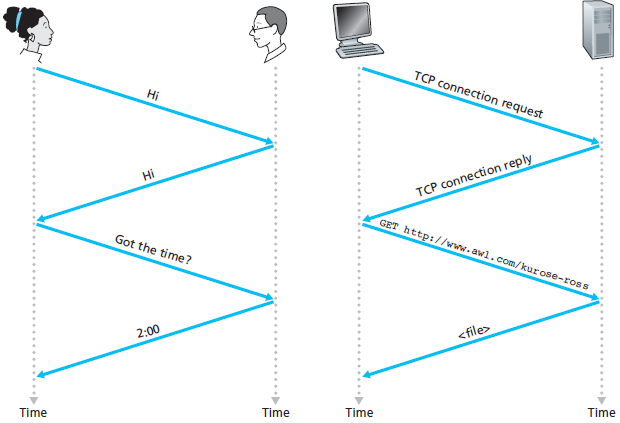
\includegraphics[width=0.5\textwidth]{./figuras/Explicacao-Protocolo.png} % <- formatos PNG, JPG e PDF
	\caption[Exemplo de Protocolo de Comunicação]{Exemplo de Protocolo de Comunicação, o paralelo entre o mecanismo de comuniacação entre humanos e um protocolo de comunicação entre máquinas exemplifica a definição de ``protocolo''.}
	\fonte{\cite{Book-Kurose2013}}
	\label{fig_explicacao_protocolo}
\end{figure}

Um protocolo de comunicação pode ser implementado em software, hardware ou em uma combinação de ambos. De maneira geral, eles são convenientemente separados em camadas ou \emph{layers}, que por sua vez oferecem ``serviços'' aos \emph{layers} superiores \cite{Book-Kurose2013}. Esses \emph{layers} são normalmente baseados em um modelo conhecido como Modelo de Referencia \sigla{OSI}{\emph{Open Systems Interconnection}} convenientemente representado na Figura \ref{fig_modelo_OSI}. Essa modularidade é extremamente útil visto que fornece um nível de abstração interessante aos protocolos, possibilitando por exemplo que o mesmo protocolo possa ser utilizado independentemente do meio físico em questão.

\begin{figure}[!htb]
	\centering
	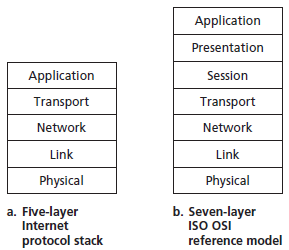
\includegraphics[width=0.4\textwidth]{./figuras/Modelo-OSI.png} % <- formatos PNG, JPG e PDF
	\caption[Modelo OSI]{Comparação entre o Modelo de Referência OSI e a pilha de protocolos de Internet.}
	\fonte{\cite{Book-Kurose2013}}
	\label{fig_modelo_OSI}
\end{figure}

%\subsection{Protocolos de Roteamento Relacionados}
Um dos protocolos de roteamento mais utilizados em Redes Locais e SGs é o \sigla{STP}{\emph{Spanning Tree Protocol}} ou \emph{Spanning Tree Protocol}. O STP recebeu este nome por ser baseado no algoritmo Prim, capaz de calcular a árvore geradora mínima de um grafo (ou \emph{spanning tree}), conforme citado em \ref{subsection-algoritmo-prim}. Ele na verdade faz parte de uma família de protocolos recorrentemente utilizados em redes de comunicação com multipercursos (caminhos redundantes). Seu principal foco é impedir a criação de \emph{loops} na rede decorrentes da topologia utilizada.

Para isso o STP utiliza pacotes especiais de controle denominados \sigla{BPDUs}{Bridge Protocol Data Units}, possibilitando que todos os equipamentos tenham o conhecimento completo da rede. De posse dessas informações, o caminho de menor custo (descrito em \ref{chap_grafos}) entre o nó raiz ou \emph{root} e os demais pode ser calculado e os comutadores então desligam as portas que não fazem parte deste caminho, criando uma topologia com um caminho único na rede para os pacotes trafegarem e impedindo a formação de \emph{loops}.

%caso necessário incluir material sobre stp

Apesar de sua configuração muitas vezes não poder ser realizada por um leigo, o STP é o protocolo mais utilizado em \emph{Smart Grids} já que possibilita a utilização de uma rede física com multi-percursos, o que significa a existência de rotas redundantes e, consequentemente, o aumento de confiabilidade/estabilidade da rede.

\section{\emph{Smart Grids} de Distribuição de Energia}
Assim como brevemente descrito no capítulo \ref{cap_introducao}, as redes inteligentes de distribuição de energia ou \emph{Smart Grids} oferecem uma ampla variedade de serviços até então minoritários ou até mesmo inexistentes nas redes de distribuição de energia convencionais. Em \cite{Art-Ma2013} pode-se encontrar um breve relato de alguns dos benefícios oferecidos pelas redes inteligentes como o melhor gerenciamento de energia, monitoramento remoto da operação e assertividade na recuperação diante de falhas, diminuição de desperdício através do maior controle entre ajuste de produção e demanda, menor necessidade de equipes de campo, entre outros. A Tabela \ref{tab_comparacao_grids} traz uma breve comparação entre os principais pontos de diferença entre as redes de comunicações utilizadas nas redes de distribuição de energia atuais e nas \emph{Smart Grids}.

\begin{table}[tbp]
\begin{tabular}{l|l|l|}
\cline{2-3}
 & \multicolumn{1}{c|}{\textbf{Grid Atual}} & \multicolumn{1}{c|}{\textbf{Smart Grid}} \\ \hline
\multicolumn{1}{|l|}{\textbf{Fluxo de informação}} & Unidirecional & Bidirecional \\ \hline
\multicolumn{1}{|l|}{\textbf{Geração de eletricidade}} & Geração centralizada & Geração Distribuída \\ \hline
\multicolumn{1}{|l|}{\textbf{Topologia do GRID}} & Radial & \emph{Mesh} \\ \hline
\multicolumn{1}{|l|}{\textbf{Sensores}} & Poucos sensores & Muitos sensores \\ \hline
\multicolumn{1}{|l|}{\textbf{Monitoramento}} & Usualmente inexistente & Auto monitorada \\ \hline
\multicolumn{1}{|l|}{\textbf{Recuperação de falha}} & Restauração manual & Auto reconfiguração \\ \hline
\multicolumn{1}{|l|}{\textbf{Teste}} & Manual & Remota \\ \hline
\multicolumn{1}{|l|}{\textbf{Capacidade de controle}} & Limitado & Penetrante \\ \hline
\multicolumn{1}{|l|}{\textbf{Tipo de controle}} & Passivo & Ativo \\ \hline
\multicolumn{1}{|l|}{\textbf{Eficiência}} & Baixa & Alta \\ \hline
\multicolumn{1}{|l|}{\textbf{Geração de poluição}} & Alta & Baixa \\ \hline
\end{tabular}
\caption[Comparação entre GRIDS normal e \emph{Smart}]{Comparação elencando os parâmetros básicos de rede entre uma rede de distribuição normal e uma rede \emph{Smart Grid}}
\fonte{Adaptado de \cite{Art-Ma2013}}
\label{tab_comparacao_grids}
\end{table}

Como dito anteriormente, os requisitos de latência das redes \emph{Smart Grid} são altamente importantes devido a multiplicidade de sensores e aplicações suportadas pela rede. \cite{Art-Deshpande2011} contém uma tabela informativa sobre os requisitos de \emph{delay} e prioridade que devem ser praticados/atingidos nestas redes destacando-se os serviços de proteção que precisam alcançar os valores de latência mais baixos sob quaisquer circunstâncias. Segundo \cite{Art-Deshpande2011} o atraso máximo para estes serviços deve ser de 10ms sob qualquer circunstância de rede, sendo este o principal fator motivador para a análise de possíveis formas de redução de latência em redes futuras onde o tráfego de dados será sensivelmente maior do que o das redes atuais.

\section{Computação Evolucional e Inteligência Artificial}
Comumente conhecida como \sigla{IA}{Inteligência Artificial} (Inteligência Artificial) ou \sigla{AI}{\emph{Artificial Intelligence}} (\emph{Artificial Intelligence}), a Inteligência Artificial pode ser considerada como um campo de pesquisa multidisciplinar ligado ao desenvolvimento e investigação de sistemas inteligentes \cite{Book-Brownlee2011}. Segundo \cite{Book-Russel2009} a IA pode ser dividida em 4 categorias: sistemas que pensam como humanos, sistemas que agem como humanos, sistemas que pensam com razão e sistemas que agem com razão.

Um dos campos comumente relacionados à IA é a Computação Evolucionária ou \sigla{CE}{Computação Evolucionária}, que foi inicialmente concebida por Lawrence J. Fogel em meados de 1960 e pode ser representada como a junção de diferentes abordagens de simulação de aspectos da evolução. Todas estas abordagens envolvem aspectos em comum como: reprodução, aleatoriedade ou mutação, competição e seleção. Até o surgimento da CE a IA estava, em sua maioria, focada em heurísticas e simulações de redes neurais primitivas. Abordagens estas que mostravam-se, segundo Fogel, limitadas já que produzem modelos muito mais próximos de um comportamento humano do que de um processo envolvido na criação de indivíduos ou intelectos (evolução) \cite{Book-Back2000}.

De maneira geral a evolução é um processo de otimização, o que definitivamente não implica em perfeição, aliado à grande robustez de adaptação visto que o mundo real nunca é estático \cite{Book-Back2000}.

Uma das classes dos algoritmos evolucionários mais difundidas e utilizadas são os Algoritmos Genéticos ou \sigla{AG}{Algoritmos Genéticos}. Estes algoritmos são caracterizados por serem uma técnica de otimização global através de estratégias adaptativas. Eles são assim chamados por serem inspirados na genética e evolução de populações e por isso se utilizam de nomenclaturas como \emph{cromossomos, genes, recombinação, mutação, etc} \cite{Book-Brownlee2011}.

\subsection{Algoritmos Genéticos}
De maneira básica e generalista pode-se dizer que uma população inicial de indivíduos devidamente correlacionados com o problema em questão é gerada, normalmente de maneira aleatória, e cada indivíduo é avaliado separadamente estabelecendo um \emph{ranking} (normalmente chamado de \emph{fitness}) dos mais adaptados ao problema sob análise. Então, alguns indivíduos da população são selecionados para reprodução, sendo que os indivíduos mais adaptados usualmente recebem mais chances de participar deste processo. Além disso, também existe a mutação que visa alterar o conteúdo genético de um indivíduo aleatoriamente, diferenciando-o de seus pais. Para o surgimento da nova geração, os indivíduos gerados (filhos) devem ser unidos aos seus pais e deve existir um método de seleção de indivíduos a fim de evitar o aumento descontrolado da população \cite{Book-Back2000}. Existem diversas técnicas diferentes para cada um dos passos acima citados, cada uma delas deve influenciar o algoritmo de maneira diferente (tempo de execução, utilização de memória, processamento utilizado, etc). Apesar de não existirem garantias, em qualquer um dos casos espera-se encontrar o valor ótimo para a função avaliada. O Algoritmo \ref{pseudocode_AG} é uma representação em alto nível da estratégia básica de um AG. 

\begin{algorithm} [h]
\caption{ - Exemplo de alto nível para AG}
\begin{algorithmic}[1]
\State $Population\gets \textit{InitializePopulation}$
\State EvaluatePopulation(Population);
\State $Sbest\gets \textit{GetBestSolution(Population)}$
\While {$ StopCondition() $}
\State $Parents\gets \textit{SelectParents(Population,PopulationSize)}$
\State $Children\gets 0$
\ForEach {$Parent1, Parent2 \in Parents $}
\State $Child1, Child2 \gets Crossover(Parent1, Parent2)$
\State $Children \gets Mutate(Child1)$
\State $Children \gets Mutate(Child2)$
\EndFor
\State EvaluatePopulation(Children);
\State $Sbest\gets \textit{GetBestSolution(Children)}$
\State $Population\gets \textit{Replace(Population,Children)}$
\EndWhile
\State\Return Sbest
\end{algorithmic}
\fonte{Adaptado de \cite{Book-Brownlee2011}}
\label{pseudocode_AG}
\end{algorithm}
